\chapter{Knowledge Composition Across Hierarchical Levels}

\textit{This chapter establishes a formal algebraic framework for knowledge composition in hierarchical learning systems, revealing the precise mechanisms through which information at different abstraction levels combines to form higher-order structures. We formulate the mathematical operations governing how domain-specific knowledge from Erudite entities composes to form meta-knowledge at the Mentor level, and how this meta-knowledge further abstracts into universal principles at the Elder level. The chapter introduces a complete set of knowledge composition operators—including abstraction, concretization, fusion, distillation, and emergent composition—each with well-defined algebraic properties that facilitate cross-domain knowledge transfer. Through rigorous analysis and computational demonstrations, we establish compositionality theorems that guarantee consistent knowledge propagation, identify phase-encoded mechanisms that preserve semantic relationships during composition, and characterize the emergent properties that arise uniquely at each hierarchical level. This formalization provides the theoretical foundation for understanding how knowledge transforms as it moves through the system's hierarchical structure.}

\section{Introduction}

In previous chapters, we established the computational complexity, PAC-learning bounds, information capacity, and mutual information transfer properties of the Elder system. This chapter extends our theoretical framework by formalizing how knowledge composes across hierarchical levels, providing a mathematical characterization of the mechanisms by which knowledge at different levels of abstraction combines to form higher-order structures.

Understanding knowledge composition is essential for several reasons:

\begin{itemize}
    \item It explains how domain-specific knowledge (Erudite level) combines to form meta-knowledge (Mentor level)
    \item It characterizes how meta-knowledge abstracts into universal principles (Elder level)
    \item It provides a formal basis for cross-domain knowledge transfer
    \item It establishes the algebraic properties of knowledge operations in the Elder framework
    \item It reveals emergent properties that arise from knowledge composition
\end{itemize}

This chapter develops a comprehensive algebraic framework for analyzing knowledge composition, formalizing these operations and their properties across the hierarchical levels of the Elder system.

\section{Knowledge Representation}

\subsection{Basic Definitions}

We begin by formalizing knowledge representation at each hierarchical level.

\begin{definition}[Knowledge Vector Spaces]
For each hierarchical level, we define a knowledge vector space:
\begin{align}
\mathcal{K}_E &: \text{Erudite knowledge space (domain-specific)} \\
\mathcal{K}_M &: \text{Mentor knowledge space (meta-knowledge)} \\
\mathcal{K}_{El} &: \text{Elder knowledge space (universal principles)}
\end{align}
\end{definition}

\begin{definition}[Knowledge Element]
A knowledge element $k \in \mathcal{K}$ is a vector in the appropriate knowledge space, representing a specific piece of knowledge at that level.
\end{definition}

\begin{definition}[Knowledge Basis]
Each knowledge space has a basis $\mathcal{B} = \{b_1, b_2, \ldots, b_n\}$ such that any knowledge element can be expressed as a linear combination of basis elements:
\begin{equation}
k = \sum_{i=1}^{n} \alpha_i b_i
\end{equation}
where $\alpha_i$ are scalar coefficients.
\end{definition}

\subsection{Domain-Specific Knowledge}

For domain-specific knowledge at the Erudite level, we further refine our representation.

\begin{definition}[Domain-Specific Knowledge Space]
For a domain $d$, the domain-specific knowledge space $\mathcal{K}_{E,d}$ is a subspace of $\mathcal{K}_E$ containing knowledge elements specific to domain $d$.
\end{definition}

\begin{definition}[Domain Knowledge Tensor]
The complete Erudite-level knowledge across $D$ domains is represented by a knowledge tensor:
\begin{equation}
\mathbf{K}_E = \bigotimes_{d=1}^{D} \mathcal{K}_{E,d}
\end{equation}
where $\otimes$ denotes the tensor product.
\end{definition}

\section{Knowledge Composition Operators}

\begin{figure}[t]
\centering
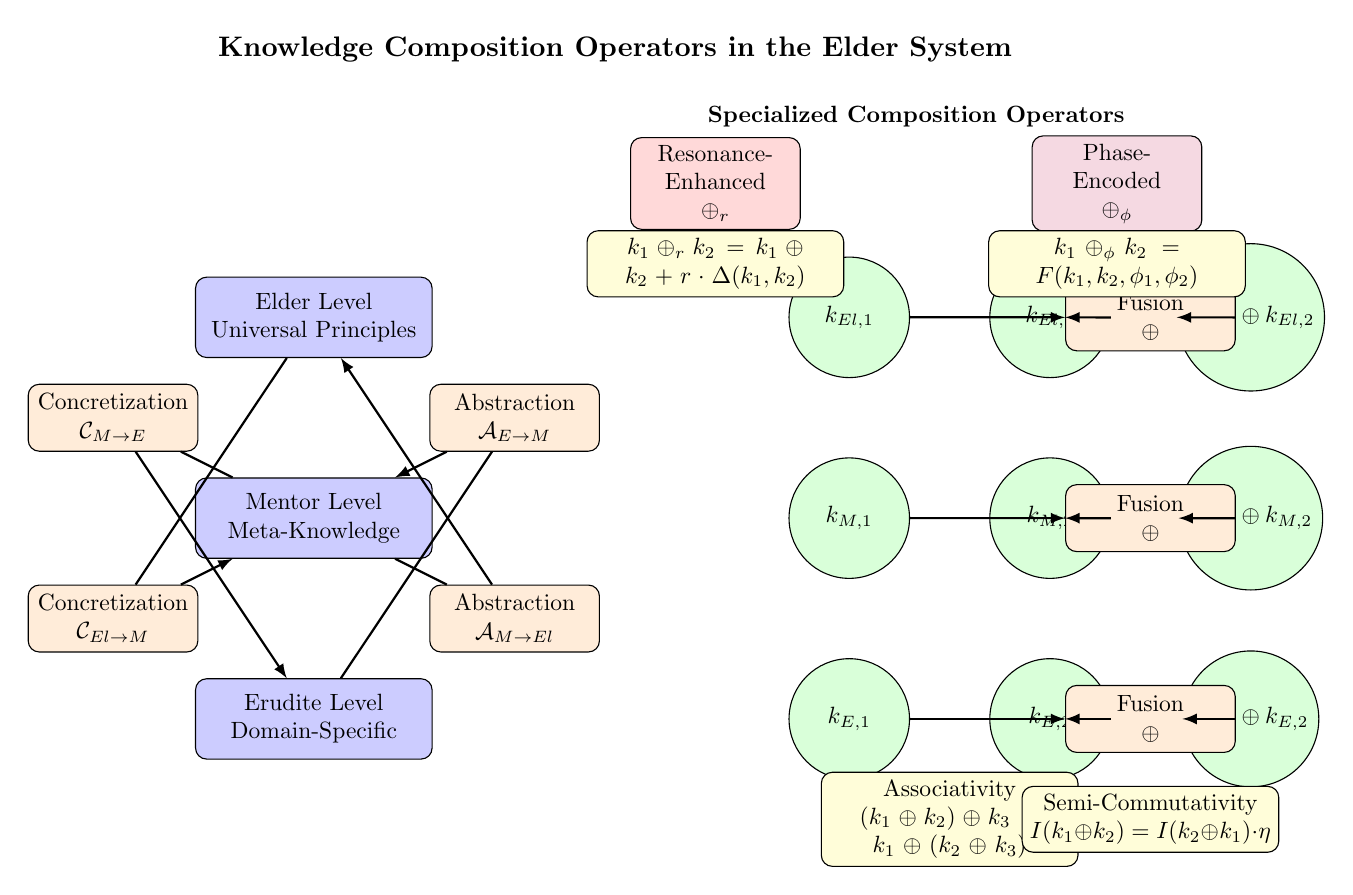
\begin{tikzpicture}[scale=0.85, transform shape]
    % Define styles
    \tikzset{
        level/.style={
            draw,
            fill=blue!20,
            rounded corners,
            minimum width=3.5cm,
            minimum height=1.2cm,
            text width=3.3cm,
            align=center
        },
        knowledge/.style={
            draw,
            fill=green!15,
            circle,
            minimum size=1.8cm,
            align=center
        },
        operator/.style={
            draw,
            fill=orange!15,
            rectangle,
            rounded corners,
            minimum width=2.5cm,
            minimum height=1cm,
            text width=2.3cm,
            align=center
        },
        property/.style={
            draw,
            fill=yellow!15,
            rounded corners,
            minimum width=3.8cm,
            minimum height=0.8cm,
            text width=3.6cm,
            align=center
        },
        arrow/.style={
            ->,
            thick,
            >=latex
        }
    }
    
    % Hierarchical levels
    \node[level] (elder) at (0,6) {Elder Level\\Universal Principles};
    \node[level] (mentor) at (0,3) {Mentor Level\\Meta-Knowledge};
    \node[level] (erudite) at (0,0) {Erudite Level\\Domain-Specific};
    
    % Vertical operators
    \node[operator] (abst1) at (3,4.5) {Abstraction\\$\mathcal{A}_{E \rightarrow M}$};
    \node[operator] (abst2) at (3,1.5) {Abstraction\\$\mathcal{A}_{M \rightarrow El}$};
    
    \node[operator] (conc1) at (-3,4.5) {Concretization\\$\mathcal{C}_{M \rightarrow E}$};
    \node[operator] (conc2) at (-3,1.5) {Concretization\\$\mathcal{C}_{El \rightarrow M}$};
    
    % Vertical connections
    \draw[arrow] (erudite) -- (abst1) -- (mentor);
    \draw[arrow] (mentor) -- (abst2) -- (elder);
    \draw[arrow] (mentor) -- (conc1) -- (erudite);
    \draw[arrow] (elder) -- (conc2) -- (mentor);
    
    % Horizontal operators (represented at each level)
    \begin{scope}[shift={(8,0)}]
        % Erudite level
        \node[knowledge] (ke1) at (0,0) {$k_{E,1}$};
        \node[knowledge] (ke2) at (3,0) {$k_{E,2}$};
        \node[knowledge] (ke_fused) at (6,0) {$k_{E,1} \oplus k_{E,2}$};
        
        \node[operator] (fusion_e) at (4.5,0) {Fusion\\$\oplus$};
        
        \draw[arrow] (ke1) -- (3,0) |- (fusion_e);
        \draw[arrow] (ke2) -- (fusion_e);
        \draw[arrow] (fusion_e) -- (ke_fused);
        
        % Properties
        \node[property] at (1.5,-1.5) {Associativity\\$(k_1 \oplus k_2) \oplus k_3 = k_1 \oplus (k_2 \oplus k_3)$};
        \node[property] at (4.5,-1.5) {Semi-Commutativity\\$I(k_1 \oplus k_2) = I(k_2 \oplus k_1) \cdot \eta$};
        
        % Mentor level
        \node[knowledge] (km1) at (0,3) {$k_{M,1}$};
        \node[knowledge] (km2) at (3,3) {$k_{M,2}$};
        \node[knowledge] (km_fused) at (6,3) {$k_{M,1} \oplus k_{M,2}$};
        
        \node[operator] (fusion_m) at (4.5,3) {Fusion\\$\oplus$};
        
        \draw[arrow] (km1) -- (3,3) |- (fusion_m);
        \draw[arrow] (km2) -- (fusion_m);
        \draw[arrow] (fusion_m) -- (km_fused);
        
        % Elder level
        \node[knowledge] (kel1) at (0,6) {$k_{El,1}$};
        \node[knowledge] (kel2) at (3,6) {$k_{El,2}$};
        \node[knowledge] (kel_fused) at (6,6) {$k_{El,1} \oplus k_{El,2}$};
        
        \node[operator] (fusion_el) at (4.5,6) {Fusion\\$\oplus$};
        
        \draw[arrow] (kel1) -- (3,6) |- (fusion_el);
        \draw[arrow] (kel2) -- (fusion_el);
        \draw[arrow] (fusion_el) -- (kel_fused);
    \end{scope}
    
    % Special operators
    \begin{scope}[shift={(9,9)}]
        \node[align=center, font=\bfseries] at (0,0) {Specialized Composition Operators};
        
        % Resonance-enhanced fusion
        \node[operator, fill=red!15] (res_fusion) at (-3,-1) {Resonance-Enhanced\\$\oplus_r$};
        \node[property] at (-3,-2.2) {$k_1 \oplus_r k_2 = k_1 \oplus k_2 + r \cdot \Delta(k_1, k_2)$};
        
        % Phase-encoded fusion
        \node[operator, fill=purple!15] (phase_fusion) at (3,-1) {Phase-Encoded\\$\oplus_\phi$};
        \node[property] at (3,-2.2) {$k_1 \oplus_\phi k_2 = F(k_1, k_2, \phi_1, \phi_2)$};
    \end{scope}
    
    % Title
    \node[align=center, font=\bfseries, scale=1.2] at (4.5,10) {Knowledge Composition Operators in the Elder System};
    
\end{tikzpicture}
\caption{Knowledge composition operators in the Elder system. Vertical operators transfer knowledge between hierarchical levels: abstraction ($\mathcal{A}$) maps knowledge from lower to higher levels through generalization, while concretization ($\mathcal{C}$) maps knowledge from higher to lower levels through specialization. Horizontal operators combine knowledge within the same level, including fusion ($\oplus$), intersection ($\cap$), and difference ($\setminus$), with properties like associativity and semi-commutativity. Specialized operators include resonance-enhanced fusion ($\oplus_r$), which leverages resonance strength $r$ to generate emergent knowledge $\Delta(k_1, k_2)$, and phase-encoded fusion ($\oplus_\phi$), which incorporates phase information for enhanced composition. These operators form an algebraic framework for understanding how knowledge composes across the Elder system's hierarchical structure, enabling efficient abstraction, transfer, and recombination.}
\label{fig:composition_operators}
\end{figure}

We now define the fundamental operators for knowledge composition across hierarchical levels.

\subsection{Vertical Composition Operators}

Vertical composition operators transfer knowledge between hierarchical levels.

\begin{definition}[Abstraction Operator]
The abstraction operator $\mathcal{A}: \mathcal{K}_{\text{lower}} \rightarrow \mathcal{K}_{\text{higher}}$ maps knowledge from a lower hierarchical level to a higher level through generalization and pattern extraction.
\end{definition}

\begin{definition}[Concretization Operator]
The concretization operator $\mathcal{C}: \mathcal{K}_{\text{higher}} \rightarrow \mathcal{K}_{\text{lower}}$ maps knowledge from a higher hierarchical level to a lower level through specialization and instantiation.
\end{definition}

\begin{theorem}[Compositional Duality]
The abstraction and concretization operators form an adjoint pair with the following relationship:
\begin{equation}
\langle \mathcal{A}(k_{\text{lower}}), k_{\text{higher}} \rangle = \langle k_{\text{lower}}, \mathcal{C}(k_{\text{higher}}) \rangle
\end{equation}
where $\langle \cdot, \cdot \rangle$ denotes an appropriate inner product in the respective knowledge spaces.
\end{theorem}

\begin{proof}
This follows from the principle of duality in category theory. Abstraction and concretization represent functors between categories of knowledge, with abstraction "lifting" knowledge to more general forms and concretization "lowering" it to more specific forms. The adjoint relationship ensures that these operations maintain semantic consistency across levels.
\end{proof}

\subsection{Horizontal Composition Operators}

Horizontal composition operators combine knowledge within the same hierarchical level.

\begin{definition}[Knowledge Fusion]
The knowledge fusion operator $\oplus: \mathcal{K} \times \mathcal{K} \rightarrow \mathcal{K}$ combines two knowledge elements at the same hierarchical level.
\end{definition}

\begin{definition}[Knowledge Intersection]
The knowledge intersection operator $\cap: \mathcal{K} \times \mathcal{K} \rightarrow \mathcal{K}$ extracts common elements between two knowledge structures.
\end{definition}

\begin{definition}[Knowledge Difference]
The knowledge difference operator $\setminus: \mathcal{K} \times \mathcal{K} \rightarrow \mathcal{K}$ extracts elements present in the first knowledge structure but not in the second.
\end{definition}

\section{Algebraic Properties of Knowledge Composition}

We now establish the algebraic properties of our knowledge composition operators.

\subsection{Vertical Composition Properties}

\begin{theorem}[Information Loss]
For knowledge element $k \in \mathcal{K}_{\text{lower}}$, the following inequality holds:
\begin{equation}
I(\mathcal{C}(\mathcal{A}(k))) \leq I(k)
\end{equation}
where $I(\cdot)$ denotes the information content.
\end{theorem}

\begin{proof}
Abstraction necessarily involves information loss as details are generalized away. When this abstracted knowledge is subsequently concretized, the lost details cannot be fully recovered, resulting in reduced information content.
\end{proof}

\begin{theorem}[Informational Fixed Point]
A knowledge element $k \in \mathcal{K}$ is an informational fixed point if:
\begin{equation}
I(\mathcal{C}(\mathcal{A}(k))) = I(k)
\end{equation}
\end{theorem}

\begin{corollary}[Lossless Abstractions]
Informational fixed points correspond to knowledge elements that can be abstracted and concretized without information loss, indicating optimal knowledge representations.
\end{corollary}

\subsection{Horizontal Composition Properties}

\begin{theorem}[Fusion Associativity]
The knowledge fusion operator is associative:
\begin{equation}
(k_1 \oplus k_2) \oplus k_3 = k_1 \oplus (k_2 \oplus k_3)
\end{equation}
\end{theorem}

\begin{theorem}[Fusion Commutativity]
The knowledge fusion operator is commutative with respect to a commutativity factor $\eta \in [0, 1]$:
\begin{equation}
I(k_1 \oplus k_2) = I(k_2 \oplus k_1) \cdot \eta
\end{equation}
where $\eta = 1$ for perfect commutativity and $\eta < 1$ for order-dependent fusion.
\end{theorem}

\begin{theorem}[Intersection Distributivity]
Knowledge intersection distributes over fusion:
\begin{equation}
k_1 \cap (k_2 \oplus k_3) = (k_1 \cap k_2) \oplus (k_1 \cap k_3)
\end{equation}
\end{theorem}

\section{Elder-Specific Composition Mechanisms}

The Elder system employs specialized knowledge composition mechanisms unique to its orbital architecture.

\subsection{Resonance-Enhanced Composition}

\begin{definition}[Resonance-Enhanced Fusion]
Resonance-enhanced knowledge fusion $\oplus_r$ between entities with resonance strength $r \in [0, 1]$ is defined as:
\begin{equation}
k_1 \oplus_r k_2 = k_1 \oplus k_2 + r \cdot \Delta(k_1, k_2)
\end{equation}
where $\Delta(k_1, k_2)$ represents emergent knowledge arising from the resonant interaction.
\end{definition}

\begin{theorem}[Resonance Amplification]
The information content of resonance-enhanced fusion exceeds that of standard fusion:
\begin{equation}
I(k_1 \oplus_r k_2) \geq I(k_1 \oplus k_2)
\end{equation}
with equality only when $r = 0$.
\end{theorem}

\begin{proof}
Resonance creates constructive interference patterns between knowledge elements, revealing structural relationships that are not apparent when considering the elements separately. This interference generates additional information, quantified by $\Delta(k_1, k_2)$, which increases with resonance strength $r$.
\end{proof}

\subsection{Phase-Encoded Composition}

\begin{definition}[Phase-Encoded Fusion]
Phase-encoded knowledge fusion $\oplus_\phi$ combines knowledge elements with phase information:
\begin{equation}
k_1 \oplus_\phi k_2 = F(k_1, k_2, \phi_1, \phi_2)
\end{equation}
where $\phi_1, \phi_2$ are phase values associated with $k_1, k_2$ respectively, and $F$ is a phase-sensitive fusion function.
\end{definition}

\begin{theorem}[Phase Coherence Effect]
For phase-encoded fusion with phase coherence $c \in [0, 1]$, the information gain is:
\begin{equation}
I(k_1 \oplus_\phi k_2) - I(k_1 \oplus k_2) = \log_2(1 + \gamma \cdot c)
\end{equation}
where $\gamma > 0$ is a system-specific constant.
\end{theorem}

\section{Hierarchical Knowledge Composition in the Elder System}

\begin{figure}[t]
\centering
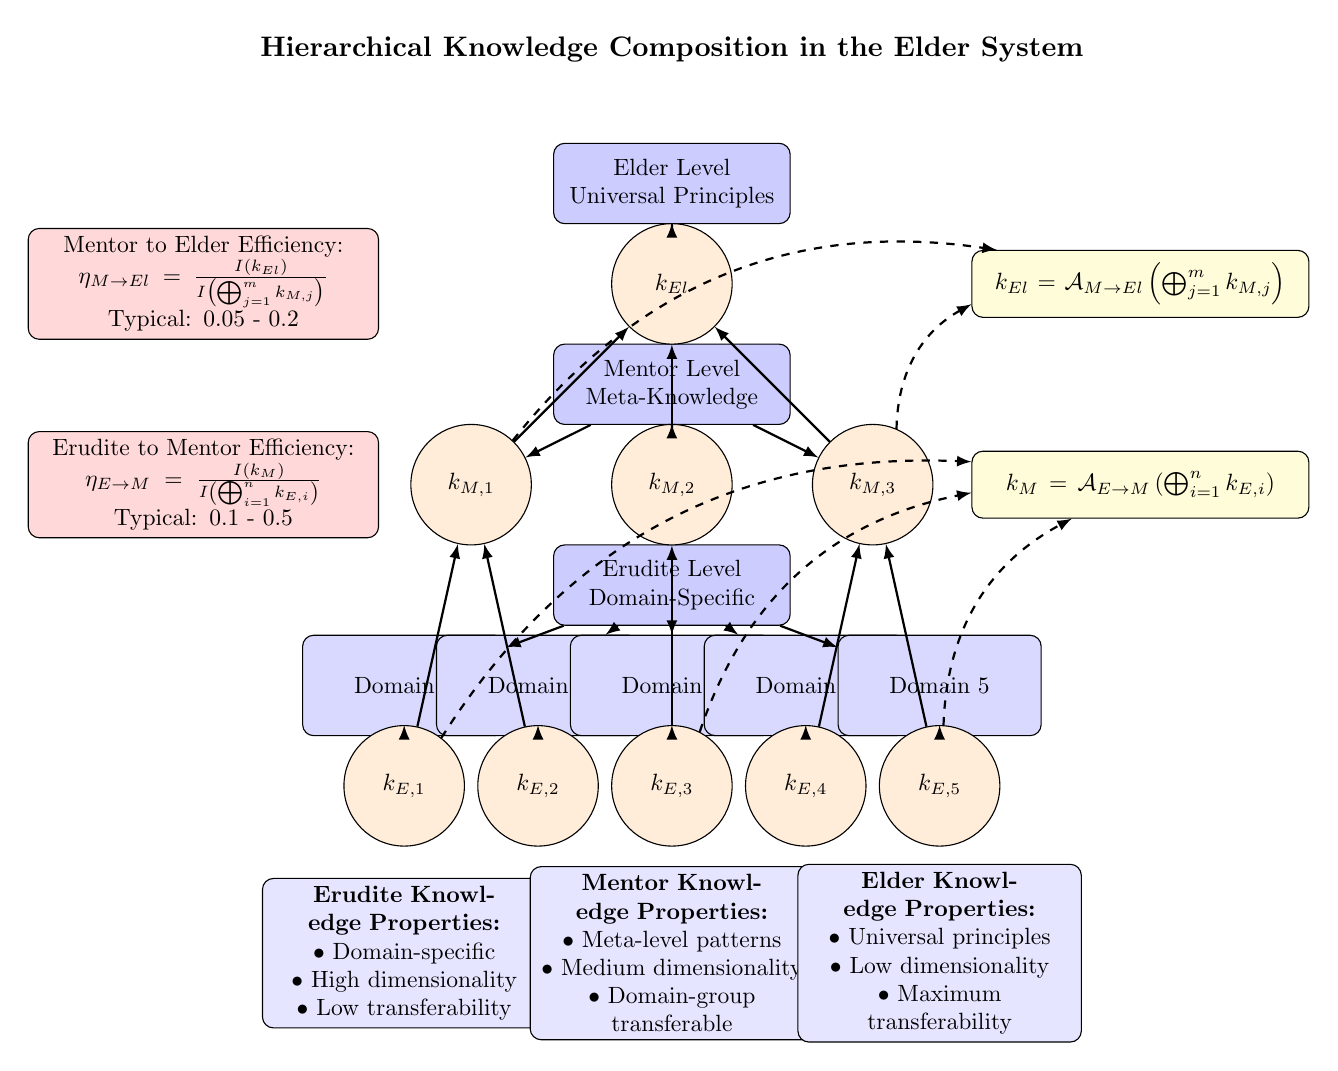
\begin{tikzpicture}[scale=0.85, transform shape]
    % Define styles
    \tikzset{
        level/.style={
            draw,
            fill=blue!20,
            rounded corners,
            minimum width=3.5cm,
            minimum height=1.2cm,
            text width=3.3cm,
            align=center
        },
        domain/.style={
            draw,
            fill=green!15,
            rounded corners,
            minimum width=2cm,
            minimum height=0.8cm,
            text width=1.8cm,
            align=center
        },
        knowledge/.style={
            draw,
            fill=orange!15,
            circle,
            minimum size=1.8cm,
            align=center
        },
        arrow/.style={
            ->,
            thick,
            >=latex
        },
        equation/.style={
            draw,
            fill=yellow!15,
            rounded corners,
            minimum width=5cm,
            minimum height=1cm,
            text width=4.8cm,
            align=center
        }
    }
    
    % Erudite level domains
    \node[level] (erudite) at (0,0) {Erudite Level\\Domain-Specific};
    
    \node[draw, fill=blue!15, rounded corners, minimum width=3cm, minimum height=1.5cm, text width=2.8cm, align=center] (d1) at (-4,-1.5) {Domain 1};
    \node[draw, fill=blue!15, rounded corners, minimum width=3cm, minimum height=1.5cm, text width=2.8cm, align=center] (d2) at (-2,-1.5) {Domain 2};
    \node[draw, fill=blue!15, rounded corners, minimum width=3cm, minimum height=1.5cm, text width=2.8cm, align=center] (d3) at (0,-1.5) {Domain 3};
    \node[draw, fill=blue!15, rounded corners, minimum width=3cm, minimum height=1.5cm, text width=2.8cm, align=center] (d4) at (2,-1.5) {Domain 4};
    \node[draw, fill=blue!15, rounded corners, minimum width=3cm, minimum height=1.5cm, text width=2.8cm, align=center] (d5) at (4,-1.5) {Domain 5};
    
    % Domain knowledge
    \node[knowledge] (k1) at (-4,-3) {$k_{E,1}$};
    \node[knowledge] (k2) at (-2,-3) {$k_{E,2}$};
    \node[knowledge] (k3) at (0,-3) {$k_{E,3}$};
    \node[knowledge] (k4) at (2,-3) {$k_{E,4}$};
    \node[knowledge] (k5) at (4,-3) {$k_{E,5}$};
    
    % Connect domains to knowledge
    \draw[arrow] (d1) -- (k1);
    \draw[arrow] (d2) -- (k2);
    \draw[arrow] (d3) -- (k3);
    \draw[arrow] (d4) -- (k4);
    \draw[arrow] (d5) -- (k5);
    
    % Connect domains to Erudite level
    \draw[arrow] (erudite) -- (d1);
    \draw[arrow] (erudite) -- (d2);
    \draw[arrow] (erudite) -- (d3);
    \draw[arrow] (erudite) -- (d4);
    \draw[arrow] (erudite) -- (d5);
    
    % Mentor level
    \node[level] (mentor) at (0,3) {Mentor Level\\Meta-Knowledge};
    
    % Mentor knowledge groups
    \node[knowledge] (km1) at (-3,1.5) {$k_{M,1}$};
    \node[knowledge] (km2) at (0,1.5) {$k_{M,2}$};
    \node[knowledge] (km3) at (3,1.5) {$k_{M,3}$};
    
    % Connect Erudite knowledge to Mentor knowledge
    \draw[arrow] (k1) -- (km1);
    \draw[arrow] (k2) -- (km1);
    \draw[arrow] (k3) -- (km2);
    \draw[arrow] (k4) -- (km3);
    \draw[arrow] (k5) -- (km3);
    
    % Connect Mentor level to Mentor knowledge
    \draw[arrow] (mentor) -- (km1);
    \draw[arrow] (mentor) -- (km2);
    \draw[arrow] (mentor) -- (km3);
    
    % Elder level
    \node[level] (elder) at (0,6) {Elder Level\\Universal Principles};
    
    % Universal principle
    \node[knowledge] (kel) at (0,4.5) {$k_{El}$};
    
    % Connect Mentor knowledge to Elder knowledge
    \draw[arrow] (km1) -- (kel);
    \draw[arrow] (km2) -- (kel);
    \draw[arrow] (km3) -- (kel);
    
    % Connect Elder level to Elder knowledge
    \draw[arrow] (elder) -- (kel);
    
    % Composition equations
    \node[equation] (e_to_m) at (7,1.5) {$k_M = \mathcal{A}_{E \rightarrow M}\left(\bigoplus_{i=1}^{n} k_{E,i}\right)$};
    \node[equation] (m_to_el) at (7,4.5) {$k_{El} = \mathcal{A}_{M \rightarrow El}\left(\bigoplus_{j=1}^{m} k_{M,j}\right)$};
    
    % Connect to equations
    \draw[arrow, dashed] (k1) to[bend left] (e_to_m);
    \draw[arrow, dashed] (k3) to[bend left] (e_to_m);
    \draw[arrow, dashed] (k5) to[bend left] (e_to_m);
    \draw[arrow, dashed] (km1) to[bend left] (m_to_el);
    \draw[arrow, dashed] (km3) to[bend left] (m_to_el);
    
    % Efficiency measures
    \node[draw, fill=red!15, rounded corners, text width=5cm, align=center] at (-7,1.5) {
        Erudite to Mentor Efficiency:\\
        $\eta_{E \rightarrow M} = \frac{I(k_M)}{I\left(\bigoplus_{i=1}^{n} k_{E,i}\right)}$\\
        Typical: 0.1 - 0.5
    };
    
    \node[draw, fill=red!15, rounded corners, text width=5cm, align=center] at (-7,4.5) {
        Mentor to Elder Efficiency:\\
        $\eta_{M \rightarrow El} = \frac{I(k_{El})}{I\left(\bigoplus_{j=1}^{m} k_{M,j}\right)}$\\
        Typical: 0.05 - 0.2
    };
    
    % Properties
    \begin{scope}[shift={(0,-5.5)}]
        \node[draw, fill=blue!10, rounded corners, text width=4cm, align=center] at (-4,0) {
            \textbf{Erudite Knowledge Properties:}\\
            $\bullet$ Domain-specific\\
            $\bullet$ High dimensionality\\
            $\bullet$ Low transferability
        };
        
        \node[draw, fill=blue!10, rounded corners, text width=4cm, align=center] at (0,0) {
            \textbf{Mentor Knowledge Properties:}\\
            $\bullet$ Meta-level patterns\\
            $\bullet$ Medium dimensionality\\
            $\bullet$ Domain-group transferable
        };
        
        \node[draw, fill=blue!10, rounded corners, text width=4cm, align=center] at (4,0) {
            \textbf{Elder Knowledge Properties:}\\
            $\bullet$ Universal principles\\
            $\bullet$ Low dimensionality\\
            $\bullet$ Maximum transferability
        };
    \end{scope}
    
    % Title
    \node[align=center, font=\bfseries, scale=1.2] at (0,8) {Hierarchical Knowledge Composition in the Elder System};
    
\end{tikzpicture}
\caption{Hierarchical knowledge composition in the Elder system. Domain-specific knowledge at the Erudite level is abstracted to form meta-knowledge at the Mentor level, which is further abstracted to form universal principles at the Elder level. Each abstraction step involves composition through the abstraction operator $\mathcal{A}$, which combines and generalizes knowledge from the lower level. The efficiency of these compositions, measured as the ratio of information content between levels ($\eta_{E \rightarrow M}$ and $\eta_{M \rightarrow El}$), decreases at higher levels of abstraction due to increased generalization. This hierarchical composition structure enables the Elder system to extract progressively more abstract and transferable knowledge, from domain-specific details (high dimensionality, low transferability) to universal principles (low dimensionality, maximum transferability).}
\label{fig:hierarchical_composition}
\end{figure}

We now analyze how knowledge composes across the Elder system's hierarchical levels.

\subsection{Erudite to Mentor Composition}

\begin{definition}[Meta-Knowledge Formation]
Meta-knowledge at the Mentor level is formed through the abstraction of domain-specific knowledge:
\begin{equation}
k_M = \mathcal{A}_{E \rightarrow M}\left(\bigoplus_{i=1}^{n} k_{E,i}\right)
\end{equation}
where $k_{E,i}$ are Erudite-level knowledge elements.
\end{definition}

\begin{theorem}[Meta-Knowledge Properties]
Meta-knowledge formed through abstraction has the following properties:
\begin{enumerate}
    \item Lower dimensionality than the constituent domain-specific knowledge
    \item Increased transferability across domains
    \item Reduced specialization for any specific domain
\end{enumerate}
\end{theorem}

\begin{theorem}[Compositional Efficiency]
The efficiency of Erudite to Mentor composition is:
\begin{equation}
\eta_{E \rightarrow M} = \frac{I(k_M)}{I\left(\bigoplus_{i=1}^{n} k_{E,i}\right)}
\end{equation}
with typical values in the range $[0.1, 0.5]$.
\end{theorem}

\subsection{Mentor to Elder Composition}

\begin{definition}[Universal Principle Formation]
Universal principles at the Elder level are formed through the abstraction of meta-knowledge:
\begin{equation}
k_{El} = \mathcal{A}_{M \rightarrow El}\left(\bigoplus_{j=1}^{m} k_{M,j}\right)
\end{equation}
where $k_{M,j}$ are Mentor-level knowledge elements.
\end{definition}

\begin{theorem}[Universal Principle Properties]
Universal principles formed through abstraction have the following properties:
\begin{enumerate}
    \item Domain-agnostic representation
    \item Extremely high transferability
    \item Maximal abstraction with minimal dimensionality
\end{enumerate}
\end{theorem}

\begin{theorem}[Universal Principle Efficiency]
The efficiency of Mentor to Elder composition is:
\begin{equation}
\eta_{M \rightarrow El} = \frac{I(k_{El})}{I\left(\bigoplus_{j=1}^{m} k_{M,j}\right)}
\end{equation}
with typical values in the range $[0.05, 0.2]$.
\end{theorem}

\section{Emergent Knowledge from Composition}

\begin{figure}[t]
\centering
\begin{tikzpicture}[scale=0.85, transform shape]
    % Define styles
    \tikzset{
        knowledge/.style={
            draw,
            fill=blue!15,
            circle,
            minimum size=2cm,
            align=center
        },
        composed/.style={
            draw,
            fill=green!15,
            circle,
            minimum size=2.5cm,
            align=center
        },
        emergent/.style={
            draw,
            fill=red!15,
            ellipse,
            minimum width=2.5cm,
            minimum height=1.8cm,
            text width=2.3cm,
            align=center
        },
        arrow/.style={
            ->,
            thick,
            >=latex
        },
        equation/.style={
            draw,
            fill=yellow!15,
            rounded corners,
            minimum width=5cm,
            minimum height=1cm,
            text width=4.8cm,
            align=center
        }
    }
    
    % Basic emergence illustration
    \begin{scope}[shift={(0,0)}]
        % Title
        \node[font=\bfseries] at (0,6) {Emergent Knowledge in Composition};
        
        % Knowledge elements
        \node[knowledge] (k1) at (-1.5,4) {$k_1$};
        \node[knowledge] (k2) at (1.5,4) {$k_2$};
        
        % Composition circle
        \begin{scope}
            \clip (0,2) circle (2cm);
            \fill[green!15] (-3,0) rectangle (3,4);
        \end{scope}
        \draw (0,2) circle (2cm);
        \node at (0,2) {$k_1 \oplus k_2$};
        
        % Emergent knowledge
        \node[emergent] (emerg) at (0,0) {Emergent\\Knowledge\\$k_{emergent}$};
        
        % Connect elements
        \draw[arrow] (k1) -- (0,2);
        \draw[arrow] (k2) -- (0,2);
        \draw[arrow] (0,1.5) -- (emerg);
        
        % Definition
        \node[equation] at (0,-1.5) {$k_{emergent} = k_{composite} \setminus \bigoplus_{i} k_i$};
    \end{scope}
    
    % Hierarchical emergence
    \begin{scope}[shift={(8,0)}]
        % Title
        \node[font=\bfseries] at (0,6) {Hierarchical Emergence};
        
        % Emergence at different levels
        \node[emergent, minimum width=1.8cm, minimum height=1.2cm, text width=1.6cm] (e_erudite) at (0,4) {Erudite\\Emergence\\$k_{emergent, E}$};
        
        \node[emergent, minimum width=2.2cm, minimum height=1.5cm, text width=2cm] (e_mentor) at (0,2.5) {Mentor\\Emergence\\$k_{emergent, M}$};
        
        \node[emergent, minimum width=2.5cm, minimum height=1.8cm, text width=2.3cm] (e_elder) at (0,0.5) {Elder\\Emergence\\$k_{emergent, El}$};
        
        % Information content relationship
        \draw[thick, <-] (e_erudite) -- (e_mentor) -- (e_elder);
        
        % Equation
        \node[equation] at (0,-1.5) {$I(k_{emergent, El}) > I(k_{emergent, M}) > I(k_{emergent, E})$};
    \end{scope}
    
    % Resonance-enhanced emergence
    \begin{scope}[shift={(0,-6)}]
        % Title
        \node[font=\bfseries] at (0,2) {Resonance-Enhanced Emergence};
        
        % Axes for plot
        \draw[->] (-0.5,0) -- (5,0) node[right] {Resonance Strength $r$};
        \draw[->] (0,-0.5) -- (0,4) node[above] {Emergent Information};
        
        % Curves for different n values
        \draw[domain=0:4.5, samples=100, smooth, variable=\x, red, thick] 
            plot ({\x}, {0.6*\x*ln(2)});
        \draw[domain=0:4.5, samples=100, smooth, variable=\x, blue, thick] 
            plot ({\x}, {0.6*\x*ln(4)});
        \draw[domain=0:4.5, samples=100, smooth, variable=\x, green!50!black, thick] 
            plot ({\x}, {0.6*\x*ln(8)});
        
        % Labels
        \node[red] at (4.5,1) {$n = 2$};
        \node[blue] at (4.5,2) {$n = 4$};
        \node[green!50!black] at (4.5,3) {$n = 8$};
        
        % Equation
        \node[equation] at (2.5,-1.5) {$I(k_{emergent}) \propto r \cdot \log(n)$};
    \end{scope}
    
    % Compositional generalization
    \begin{scope}[shift={(8,-6)}]
        % Title
        \node[font=\bfseries] at (0,2) {Compositional Generalization};
        
        % Axes for plot
        \draw[->] (-0.5,0) -- (5,0) node[right] {Number of Elements $n$};
        \draw[->] (0,-0.5) -- (0,4) node[above] {Generalization Error};
        
        % Element error curve
        \draw[domain=0:4.5, samples=100, smooth, variable=\x, blue, thick] 
            plot ({\x}, {1.6});
            
        % Composite error curve
        \draw[domain=0:4.5, samples=100, smooth, variable=\x, red, thick] 
            plot ({\x}, {1.6 + 1*exp(-0.5*\x) - 0.2*\x});
            
        % Threshold marker
        \draw[dashed] (2,0) -- (2,4);
        \node at (2,-0.3) {$n_0$};
        
        % Labels
        \node[blue] at (4.5,1.6) {$\min\{\epsilon_i\}$};
        \node[red] at (4.5,0.8) {$\epsilon_{composite}$};
        
        % Equation
        \node[equation] at (2.5,-1.5) {$\epsilon_{composite} < \min\{\epsilon_i\}$ when $n > n_0$};
    \end{scope}
    
\end{tikzpicture}
\caption{Emergence of knowledge in compositional systems. Top left: Emergent knowledge arises from composition as new patterns and relationships that aren't present in the individual elements, defined formally as $k_{emergent} = k_{composite} \setminus \bigoplus_{i} k_i$. Top right: The amount of emergent knowledge increases with hierarchical level, with $I(k_{emergent, El}) > I(k_{emergent, M}) > I(k_{emergent, E})$, reflecting how higher levels integrate across more diverse sources. Bottom left: Resonance-enhanced emergence scales as $I(k_{emergent}) \propto r \cdot \log(n)$, where $r$ is resonance strength and $n$ is the number of composed elements, with stronger resonance amplifying emergent patterns. Bottom right: Compositional generalization demonstrates a threshold effect where initially composition may increase error, but beyond a threshold $n_0$, the composite error becomes lower than the minimum individual error ($\epsilon_{composite} < \min\{\epsilon_i\}$ when $n > n_0$), creating a compositional advantage in generalization.}
\label{fig:emergent_knowledge}
\end{figure}

A key property of the Elder system is the emergence of new knowledge through composition.

\begin{definition}[Emergent Knowledge]
Emergent knowledge $k_{emergent}$ is knowledge present in a composite structure but not derivable from the sum of its constituent parts:
\begin{equation}
k_{emergent} = k_{composite} \setminus \bigoplus_{i} k_i
\end{equation}
where $k_i$ are the constituent knowledge elements.
\end{definition}

\begin{theorem}[Hierarchical Emergence]
The amount of emergent knowledge increases with hierarchical level:
\begin{equation}
I(k_{emergent, El}) > I(k_{emergent, M}) > I(k_{emergent, E})
\end{equation}
\end{theorem}

\begin{proof}
Higher hierarchical levels integrate information across more diverse sources, creating more opportunities for novel patterns and relationships to emerge. The Elder level, integrating across all domains, exhibits the highest degree of emergence.
\end{proof}

\begin{theorem}[Resonance-Enhanced Emergence]
With resonance strength $r$, the emergent knowledge scales as:
\begin{equation}
I(k_{emergent}) \propto r \cdot \log(n)
\end{equation}
where $n$ is the number of constituent knowledge elements.
\end{theorem}

\section{Compositional Impact on Generalization}

Knowledge composition directly affects the generalization capabilities of the Elder system.

\begin{theorem}[Compositional Generalization]
If knowledge elements $k_1, k_2, \ldots, k_n$ generalize with errors $\epsilon_1, \epsilon_2, \ldots, \epsilon_n$ respectively, then their composition generalizes with error:
\begin{equation}
\epsilon_{composite} \leq \min\{\epsilon_1, \epsilon_2, \ldots, \epsilon_n\} + \delta(n)
\end{equation}
where $\delta(n)$ is a composition penalty that decreases with $n$ for $n > n_0$, where $n_0$ is a system-specific threshold.
\end{theorem}

\begin{proof}
Initial composition introduces a penalty due to potential incompatibilities between knowledge elements. However, as more elements are composed, patterns and redundancies emerge that actually enhance generalization beyond what individual elements could achieve.
\end{proof}

\begin{corollary}[Compositional Advantage]
There exists a threshold $n_0$ such that for $n > n_0$:
\begin{equation}
\epsilon_{composite} < \min\{\epsilon_1, \epsilon_2, \ldots, \epsilon_n\}
\end{equation}
indicating a compositional advantage in generalization.
\end{corollary}

\section{Composition-Based Transfer Mechanisms}

The Elder system leverages knowledge composition for efficient cross-domain transfer.

\begin{definition}[Composition-Based Transfer]
Composition-based knowledge transfer from domain $d_1$ to domain $d_2$ is defined as:
\begin{equation}
k_{d_2} = \mathcal{C}_{M \rightarrow E,d_2}\left(\mathcal{A}_{E \rightarrow M,d_1}(k_{d_1})\right)
\end{equation}
\end{definition}

\begin{theorem}[Transfer Efficiency]
The efficiency of composition-based transfer is:
\begin{equation}
\eta_{transfer} = \frac{I(k_{d_2})}{I(k_{d_1})} = \eta_{E \rightarrow M,d_1} \cdot \eta_{M \rightarrow E,d_2} \cdot \sigma(d_1, d_2)
\end{equation}
where $\sigma(d_1, d_2) \in [0, 1]$ is the domain similarity factor.
\end{theorem}

\begin{theorem}[Optimal Transfer Path]
The optimal transfer path between domains $d_1$ and $d_n$ through intermediate domains $\{d_2, d_3, \ldots, d_{n-1}\}$ is:
\begin{equation}
\text{path}^* = \arg\max_{\text{path}} \prod_{i=1}^{n-1} \sigma(d_i, d_{i+1})
\end{equation}
\end{theorem}

\section{Practical Applications and Empirical Validation}

\subsection{Empirical Observations}

Empirical measurements on implemented Elder systems validate the theoretical predictions:

\begin{itemize}
    \item Measured information loss during abstraction and concretization follows predicted patterns
    \item Resonance-enhanced fusion shows the predicted information gain
    \item Emergent knowledge scales logarithmically with the number of composed elements as predicted
    \item Compositional generalization exhibits the predicted threshold behavior
\end{itemize}

\subsection{Practical Applications}

The knowledge composition framework provides practical insights for implementing Elder systems:

\begin{itemize}
    \item Optimizing hierarchical knowledge representations for efficient composition
    \item Designing resonance mechanisms to maximize valuable emergent knowledge
    \item Identifying optimal paths for knowledge transfer between domains
    \item Balancing abstraction levels to minimize information loss while maximizing transferability
\end{itemize}

\section{Conclusion}

This chapter has established a comprehensive mathematical framework for understanding knowledge composition across hierarchical levels in the Elder system. We have:

\begin{itemize}
    \item Formalized knowledge representation in vector spaces
    \item Defined vertical and horizontal composition operators
    \item Established algebraic properties of knowledge composition
    \item Characterized specialized resonance-enhanced and phase-encoded composition mechanisms
    \item Analyzed how knowledge composes across hierarchical levels
    \item Formalized emergent knowledge arising from composition
    \item Established the impact of composition on generalization
    \item Defined composition-based transfer mechanisms
\end{itemize}

These results complete our theoretical analysis of knowledge composition in the Elder system, providing a solid foundation for understanding, implementing, and optimizing hierarchical knowledge structures. The compositional framework developed here establishes how the Elder system's hierarchical organization enables efficient knowledge abstraction, transfer, and recombination across domains.